s]\chapter{Inside \texorpdfstring{$\epsilon_0$}{epsilon0}: The Ketonen-Solovay machinery\label{ks-chapter}}
\label{chap:ketonen}
\index{Maths!Ketonen-Solovay machinery}

\section{Introduction}
The reader may think that our proof of termination in the previous  chapter requires a lot of mathematical tools and may be too  complex. So, the question is ``is there  any  simpler proof'' ?

In their article~\cite{KP82}, Kirby and Paris show that this result cannot be proved in Peano arithmetic. Their proof uses some knowledge about model theory and non-standard models of Peano arithmetic. In this chapter, we focus on a specific class of proofs of termination of hydra battles: construction of some variant mapping the type \texttt{Hydra} into some segment of ordinals. Our proof relies only on the Calculus of Inductive Constructions and is a natural complement of the results proven in the previous chapter.

\begin{itemize}
\item There is no variant mapping the type \texttt{Hydra} into the interval $[0,\omega^2[$ (section ~\vref{omega2-case}), and a fortiori 
$[0,\omega[$

\item There is a variant that maps the type \texttt{Hydra} into the
interval $[0,\epsilon_0[$ (theorem \texttt{every\_battle\_terminates}, in section~\vref{hydra-variant}).
\end{itemize}


Thus, a very natural question is the following one:
\begin{quote}
  `` Is there  any variant from
\texttt{Hydra} into some interval $[0,\mu[$, where $\mu<\epsilon_0$, for proving the termination of all hydra battles ?''
\end{quote}

We prove in \coq{} the following results:

\begin{quote}
There is no variant for proving the termination of all hydra battles
from \texttt{Hydra} into the interval $[0..\mu[$, where
$\mu< \epsilon_0$.
The same impossibility holds even if we consider only standard battles (with the successive replication factors $0,1,2,\dots,t,t+1,\dots$).
\end{quote}

Our proofs are  constructive and require no axioms: they are  closed terms of the CIC, and are mainly composed on function definitions and proofs of properties of these functions. 
They  share much theoretical material with Kirby and Paris', although they do not use any knowledge about Peano arithmetic nor model  theory.  The combinatorial arguments we use and implement
come from 
 an article by J.~Ketonen and R.~Solovay~\cite{KS81}, already  cited in the work
 by L.~Kirby et J.~Paris on the termination of Goodstein sequences and hydra battles~\cite{KP82}.
 Section $2$ of this article: ''A hierarchy of probably recursive functions'', contains a systematic study of \emph{canonical sequences}, which are closely related to
rounds of hydra battles. 



\section{Canonical Sequences}
\label{ketonen-solovay-sect}
\index{Maths!Canonical sequences}

Canonical sequences are functions that associate an ordinal $\canonseq{\alpha}{i}$ to every ordinal $\alpha<\epsilon_0$ and positive integer $i$. They satisfy nice properties :

\index{Maths!Transfinite induction}
\begin{itemize}
\item If $\alpha\not=0$, then $\canonseq{\alpha}{i}<\alpha$. Thus canonical sequences can be used for proofs by transfinite induction or function definition by transfinite recursion
\item If $\lambda$ is a limit ordinal, then $\lambda$ is the least upper bound of the set 
$\{\canonseq{\lambda}{i}\;|\,i\in\mathbb{N}_1\}$


\item If $\beta<\alpha<\epsilon_0$, then there is a ``path'' from $\alpha$ to $\beta$, \emph{i.e.} a
sequence $\alpha_0=\alpha, \alpha_1, \dots, \alpha_n=\beta$, where for every $k<n$, there exists some $i_k$ such that $\alpha_{k+1}=\canonseq{\alpha_k}{i_k}$
\item Canonical sequences correspond tightly to rounds of hydra battles: if $\alpha\not=0$,
then $\iota(\alpha)$ is transformed into $\iota(\canonseq{\alpha}{i+1}$ in one round with
the replication factor $i$ (Lemma \href{../src/html/hydras.Hydra.O2H.html\#canonS_iota_i}{Hydra.O2H.canonS\_iota\_i}).
\item From the two previous properties, we infer that whenever $\beta<\alpha<\epsilon_0$, there exists a (free) fight from $\iota(\alpha)$ to $\iota(\beta)$.
\end{itemize}

\paragraph{Remark}
In~\cite{KS81}, canonical sequences are defined for any ordinal $\alpha <\epsilon_0$,
by stating that if $\alpha$ is a successor ordinal, the sequence associated with 
$\alpha$ is simply the constant sequence whose terms are equal to the predecessor of $\alpha$. Likewise, we define the canonical sequence of $0$ as the
sequence whose all terms are equal to $0$.

This convention allows us to make total the function that maps any ordinal $\alpha$ and natural number $i$ to the $i$-th item of the canonical sequence associated with $\alpha$.


First, let us recall how canonical sequences are defined in~\cite{KS81}. For efficiency's sake, we decided not to implement directly K.\&S's definitions, but to define in \gallina{} simply typed structurally recursive functions which share the abstract properties which are used in the mathematical proofs\footnote{With a small diffrence: the $0$-th term of the canonical sequence is not the same in our development as in~\cite{KS81}.}





\subsubsection{Mathematical definition of canonical sequences} 





In~\cite{KS81} the definition of $\canonseq{\alpha}{i}$ is based on the following remark:
\begin{quote}
Any non-zero ordinal $\alpha$ can be decomposed in a unique way as the product
$\omega^\beta\times (\gamma+1)$.
\end{quote}

Thus the $\canonseq{\alpha}{i}$\,s are defined in terms of this decomposition:
\begin{definition}[Canonical sequences: mathematical definition]
\label{def:canonseq-math}
  
\end{definition}
\begin{mathframe}
  \begin{itemize}
\item Let $\lambda<\epsilon_0$ be a limit ordinal 

\begin{itemize}
\item If $\lambda=\omega^{\alpha+1}\times (\beta+1)$, then 
$\canonseq{\lambda}{i}= \omega^{\alpha+1}\times\beta +  \omega^\alpha \times i$
\item If $\lambda=\omega^{\gamma}\times (\beta+1)$, where $\gamma<\lambda$ is a limit ordinal, then 
$\canonseq{\lambda}{i}=\omega^{\gamma}\times \beta + \omega^{\canonseq{\gamma}{i}}$
\end{itemize}

\item For successor ordinals, we have $\canonseq{\alpha+1}{i}= \alpha$ 

\item Finally, $\canonseq{0}{i}= \alpha$.
\end{itemize}
\end{mathframe}

\subsubsection{Canonical sequences in Coq}

Our definition may look more complex than the mathematical one, but
uses plain structural recursion over the type \coqsimple{T1}. Thus, tactics like
\coqsimple{cbn}, \coqsimple{simpl}, \coqsimple{compute}, etc., are applicable. For simplicity's sake, 
we used an auxiliary function \texttt{canonS} of type \texttt{T1 -> nat  -> T1} such that
\texttt{canonS  $\alpha$ $i$} is equal to $\canonseq{\alpha}{i+1}$.

\vspace{4pt}
\emph{From Module~\href{../src/html/hydras.Epsilon0.Canon.html\#canonS}{Epsilon0.Canon}}

\index{Functions!canonS canonS (helper for canon)}
\index{Functions!canon @ canon (canonical sequence)}
\begin{Coqsrc}
Fixpoint canonS alpha (i:nat) :=
  match alpha with
      zero => zero
    | ocons zero 0 zero => zero
    | ocons zero (S k) zero => FS k
    | ocons gamma 0 zero =>
      match pred gamma with
          Some gamma' => ocons gamma' i zero
        | None => ocons (canonS gamma i) 0 zero
      end
    | ocons gamma (S n) zero =>
       match pred gamma with
           Some gamma' => ocons gamma n (ocons gamma' i zero)
         | None => ocons gamma n (ocons (canonS gamma i) 0 zero)
       end
    | ocons alpha n beta => ocons alpha n (canonS beta i)
  end.
\end{Coqsrc}


The following function computes $\canonseq{\alpha}{i}$, except for the case $i=0$, where it simply returns $0$\;\footnote{This restriction did not prevent us from proving all the main theorems of~\cite{KS81, KP82}. Nevertheless, in a future version of this development, we may define $\canonseq{\alpha}{0}$ exactly as 
in~\cite{KS81}. This would  be done at the cost of making proofs much more complex.}.

\begin{Coqsrc}
 Definition canon alpha i := 
   match i with 0 => zero | S j => canonS alpha j end. 
\end{Coqsrc}

For instance \coq's computing facilities allow us to verify the equalities\linebreak 
\mathcolor{$\canonseq{\omega^\omega}{3} = \omega^3$} and
\mathcolor{$\canonseq{\omega^\omega*3}{42} = \omega^\omega*2 + \omega^{42}$}.


\begin{Coqsrc}
Compute (canon (omega ^ omega) 3).
\end{Coqsrc}

\begin{Coqanswer}
  = phi0 (FS 2) : T1
\end{Coqanswer}

\begin{Coqsrc}
Example canon3 :  canon (omega ^ omega) 3 = omega ^ 3.
Proof. reflexivity. Qed.
\end{Coqsrc}


\begin{Coqsrc}
Compute pp (canon (omega ^ omega * 3) 42).  
\end{Coqsrc}

\begin{Coqanswer}
    = (omega ^ omega * 2 + omega ^ 42)%pT1
     : ppT1
\end{Coqanswer}

\subsection{Basic properties of canonical sequences}

We did not  try to prove that our definition really implements Ketonen and Solovay's  \cite{KS81}'s canonical sequences. The most important is that we were able to prove the 
abstract properties  of canonical sequences that are really used in our proof. The complete proofs are in the module
~\href{../src/html/hydras.Epsilon0.Canon.html}{Epsilon0.Canon}


Proving the equality $\canonseq{\alpha+1}{i}=\alpha$ is not 
as simple as suggested by the equations of definition~\ref{def:canonseq-math}\,.
Nevertheless, we could prove it by  structural induction on $\alpha$.

\begin{Coqsrc}
Lemma canonS_succ i alpha :
  nf alpha ->  canonS (succ alpha) i = alpha.
Proof.
 induction alpha.
 (* ... *)
\end{Coqsrc}

\subsubsection{Canonical sequences and the order $<$}

\index{Maths!Transfinite induction}

First, we prove by transfinite induction over $\alpha$ that $\canonseq{\alpha}{i+1}$ is an ordinal strictly less than $\alpha$ (assuming $\alpha\not=0$). This property allows us to use the function \texttt{canonS} and its derivates in function definitions by transfinite recursion.

\label{lemma:canonS_LT}
\begin{Coqsrc}
Lemma canonS_LT i alpha :
  nf alpha -> alpha <> zero -> canonS alpha i <  alpha.
\end{Coqsrc}


\subsubsection{Limit ordinals are really limits}
The following theorem states that any limit ordinal $\lambda<\epsilon_0$ 
is the limit of the sequence \showmath{\canonseq{\lambda}{i}\;(1\le i)}.

Note the use of \coq's \texttt{sig} type in the theorem's statement, which
relates the boolean function \texttt{is\_limit} defined on the \texttt{T1} data-type with a constructive view of the limit of a sequence: for any $\beta<\lambda$, we can compute an item of the canonical sequence of $\lambda$ which is greater than $\beta$.


\vspace{4pt}
\emph{From Module~\href{../src/html/hydras.Epsilon0.Canon.html\#canonS_limit_strong}{Epsilon0.Canon}}


\begin{Coqsrc}
Lemma canonS_limit_strong (lambda : T1) : 
     nf lambda ->
     limitb lambda  ->
     forall beta, beta < lambda ->
                  {i:nat | beta < canonS lambda i}.

Proof.
  transfinite_induction_LT lambda.
  (* ... *)
Defined.
\end{Coqsrc}

\label{lemma:canonS-limit}

\begin{Coqsrc}
Lemma canonS_limit_lub (lambda : T1) :
  nf lambda -> limitb lambda  ->
  strict_lub (fun i => canonS lambda i) lambda.
\end{Coqsrc}

\index{Exercises}

\begin{exercise}\label{exo:simply-typed-canonseq}
Instead of using the \texttt{sig} type, define a simply typed function that, given two ordinals $\alpha$ and $\beta$, returns a natural number $i$ such that, if $\alpha$ is a limit ordinal and $\beta<\alpha$, then $\beta< \canonseq{\alpha}{i+1}$. Of course, you will have to prove the correctness of your function.
\end{exercise}




\section{Accessibility inside \texorpdfstring{$\epsilon_0$}{epsilon0} : Paths}
\index{Maths!Accessibility inside epsilon0}

Let us consider a kind of accessibility problem inside $\epsilon_0$: given two ordinals $\alpha$ and $\beta$, where $\beta<\alpha<\epsilon_0$, find a \emph{path} consisting of a finite sequence $\gamma_0=\alpha,\dots,\gamma_l=\beta$,
where, for every $i<l$, $\gamma_i \not= 0$ and there exists some strictly positive integer $s_i$
such that $\gamma_{i+1}=\canonseq{\gamma}{s_i})$,

\subsection{Definition}

We shall denote by $\alpha\xrightarrow [s]{}\beta$
  the proposition 
``there is a path from $\alpha$ to $\beta$ with $s$ as the sequence of indices
$s_0,s_1,\dots,s_{l-1}$ ''.

For instance, we have $\omega*2 \xrightarrow[2,2,2]{}\omega$, through the 
sequence of ordinals $\omega\times 2, \omega+2,\omega+1,\omega$.



Note that, given $\alpha$ and $\beta$, where $\beta < \alpha$, the sequence $s$ which leads from $\alpha$ to $\beta$ is not unique.

Indeed, if $\alpha$ is a limit ordinal, the first element of $s$ can be any integer $i$ such that $\beta<\canonseq{\alpha}(i)$, and if $\alpha$ is a successor ordinal,
then the sequence $s$ can start with any positive integer.


For instance, we have also 
$\omega*2 \xrightarrow[3,4,5,6]{}\omega$. 
Likewise,
$\omega*2 \xrightarrow[{[3,14]}]{} 0$ and
$\omega*2 \xrightarrow[s] 0$, where $s$ is the sequence containing eight times the number $3$.

\label{path-to-definition}

In \coq{}, the notion of path can be simply defined as an inductive predicate 
parameterized by the destination $\beta$.

\vspace{4pt}
\emph{From Module~\href{../src/html/hydras.Epsilon0.Paths.html}{Epsilon0.Paths}}


\begin{Coqsrc}
(Definition transition_S i : relation T1 :=
  fun alpha beta =>  alpha <> zero /\ beta = canonS alpha i.

Definition transition i : relation T1 :=
  match i with 0 => fun _ _ => False | S j => transition_S j end.
\end{Coqsrc}

\index{Predicates!path\_to}

\begin{Coqsrc}
Inductive path_to (beta: T1) : list nat -> T1 -> Prop :=
  path_to_1 : forall (i:nat) alpha , 
    i <> 0 ->
    transition i alpha beta ->
    path_to beta (i::nil) alpha
| path_to_cons : forall i alpha s gamma,
    i <> 0 ->
    transition i alpha gamma ->
    path_to beta  s gamma ->
    path_to beta  (i::s) alpha.
\end{Coqsrc}





\begin{remark}
In the present version of our library, we use a variant \texttt{path\_toS} of
\texttt{path\_to}, where the proposition
(\texttt{path\_toS $\beta$ $s$ $\alpha$}) is equivalent to
(\texttt{path\_to $\beta$ (shift $s$) $\alpha$}). This variant is scheduled to be deprecated.
\end{remark}

\index{Exercises}

\begin{exercise}
Write a tactic for solving goals of the form (\texttt{path\_to $\beta$ $s$ $\alpha$})
where $\alpha$, $\beta$ and $s$ are closed terms. 
You should solve automatically the following goals:

\begin{Coqsrc}
 path_to omega (2::2::2::nil) (omega * 2).

 path_to omega (3::4::5::6::nil) (omega * 2).

 path_to zero (interval 3 14) (omega * 2).

 path_to zero (repeat 3 8) (omega * 2).
\end{Coqsrc}

\end{exercise}

\subsection{Existence of a path}

\index{Maths!Transfinite induction}

By transfinite induction on $\alpha$, we prove that for any $\beta<\alpha$, 
on can build a path from $\alpha$ to $\beta$.

\begin{Coqsrc}
Lemma LT_path_to (alpha beta : T1) :
  beta < alpha -> {s : list nat | path_to beta s alpha}.
\end{Coqsrc}

\index{Exercises}

\begin{exercise}[Continuation of exercise~\vref{exo:simply-typed-canonseq}]
Define a simply typed function for computing a path from $\alpha$ to $\beta$.
\end{exercise}

% ici
\noindent 
From the lemma \texttt{canonS\_LT}~\vref{lemma:canonS_LT}, we convert any path into an inequality on ordinals (by induction on paths).


\begin{Coqsrc}
Lemma path_to_LT beta s alpha :
  path_to beta s alpha -> nf alpha -> beta < alpha.
\end{Coqsrc}

\subsection{Paths and hydra battles}
\label{KS-o2h}

In order to apply our knowledge about  ordinal numbers (less than $\epsilon_0$) to the study of hydra battles, we define an injection
from the interval $[0,\epsilon_0[$ into the type \texttt{Hydra}.

\vspace{4pt}

\emph{From Module~\href{../src/html/hydras.Hydra.O2H.html}{Hydra.O2H}}


\begin{Coqsrc}
Fixpoint iota (alpha : T1) : Hydra :=
  match alpha with
  | T1.zero => head
  | ocons gamma n beta => 
         node (hcons_mult (iota gamma) (S n) (iotas beta))
  end 
with iotas (alpha : T1) :  Hydrae :=
       match alpha with
       | T1.zero => hnil
       | ocons alpha0 n beta  => 
           hcons_mult (iota alpha0) (S n)
                                (iotas beta)
       end.
\end{Coqsrc}  




For instance Fig.~\ref{fig:iota-example} shows the image by $\iota$ of the ordinal  \textcolor{black}{$\omega^{\omega+2}+\omega^\omega \times 2 + \omega + 1$}

  \begin{figure}[htb]
\centering
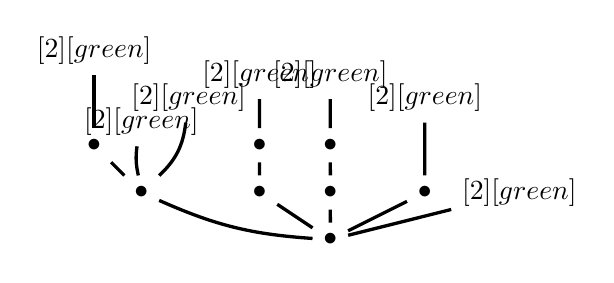
\begin{tikzpicture}[very thick, scale=0.3]
\node (foot) at (10,0) {$\bullet$};
\node (N1) at (2,2) {$\bullet$};
\node (N2) at (10,2) {$\bullet$};
\node (N22) at (7,2) {$\bullet$};
\node (N3) at (14,2) {$\bullet$};
\node (N4) at (18,2) {$\Smiley[2][green]$};
\node (N5) at (0,4) {$\bullet$};
\node (N6) at (2,5) {$\Smiley[2][green]$};
\node (N7) at (4,6) {$\Smiley[2][green]$};
\node (N88) at (7,4) {$\bullet$};
\node (N8) at (10,4) {$\bullet$};
\node (N9) at (14,6) {$\Smiley[2][green]$};
\node (N10) at (0,8) {$\Smiley[2][green]$};
\node (N11) at (10,7) {$\Smiley[2][green]$};
\node (N111) at (7,7) {$\Smiley[2][green]$};
\draw (foot) to [bend left=10] (N1);
\draw (foot) -- (N2);
\draw (foot) -- (N22);
\draw (foot) -- (N3);
\draw (foot) -- (N4);
\draw (N1) to  (N5);
\draw (N1) to   [bend left=10] (N6);
\draw (N1) to   [bend right=20] (N7);
\draw (N2) to  (N8);
\draw (N22) to  (N88);
\draw (N8) to  (N11);
\draw (N88) to  (N111);
\draw (N3) to  (N9);
\draw (N5) to  (N10);
\end{tikzpicture}
\caption{The hydra $\iota(\omega^{\omega+2}+\omega^\omega \times 2 + \omega + 1$) \label{fig:iota-example}}

\end{figure}


The following lemma (proved in ~\href{../src/html/hydras.Hydra.O2H.html}{Hydra.O2H.v}) maps  canonical sequences to rounds of hydra battles.


\label{lemma:canonS-iota}

\begin{Coqsrc}
Lemma canonS_iota i alpha :
    nf alpha -> alpha <> 0 ->
    iota alpha -1-> iota (canonS alpha i).
\end{Coqsrc}
                

The next step of our development is to extend this relationship to
the order $<$ on $[0,\epsilon_0[$ on one side, and hydra fights on the other side.

\begin{Coqsrc}
Lemma path_to_fight alpha s beta :
  path_to  beta  s alpha -> nf alpha ->
  iota alpha -+-> iota beta.
\end{Coqsrc}

As a corollary, we are now able to transform any inequality $\beta<\alpha<\epsilon_0$ into a (free) fight.

\begin{Coqsrc}
Lemma LT_to_fight alpha beta :
    beta < alpha ->  iota alpha -+-> iota beta.
\end{Coqsrc}

\section{A first proof of impossibility}

We have got all the tools for proving there is no variant bounded by some $\mu<\epsilon_0$ for proving the termination   of all battles. The proof we are going to show is a proof by contradiction. It  can
 be considered as a generalization of the
proofs described in  sections~\vref{omega-case} and \vref{omega2-case}.
We advise the reader to compare the three proofs step by step, lemma by lemma.


In the module \href{../src/html/hydras.Hydra.Epsilon0_Needed_Generic.html}{Hydra.Epsilon0\_Needed\_Generic}, we assume there exists some variant $m$ bounded by some ordinal $\mu<\epsilon_0$. This part of the development is parameterized by some class $B$ of battles, which will be instantiated later to \texttt{free} or \texttt{standard}.


\index{Coq!Techniques!Type classes}

\begin{Coqsrc}
Class BoundedVariant  (B:Battle) :=
  {
    mu:T1 ;
    m: Hydra -> T1;
    mu_nf : nf mu;
    Hvar : Hvariant T1_wf B m;
    m_bounded : forall h, m h < mu
  }.
\end{Coqsrc}

Let us assume there exists such a variant:

\begin{Coqsrc}
Section Bounded.
  Context (B: Battle)  (Hy : BoundedVariant B).

  Hypothesis m_decrease : forall  i h h',
        round_n i h h' -> m h' < m h.
\end{Coqsrc}

\begin{remark}
  The hypothesis \texttt{m\_decrease} is false in general, but is satisfied by
the  \texttt{free} and \texttt{standard} kinds of battles. This trick allows to 
``factorize'' our proofs our proofs of impossibility.
\end{remark}

\index{Maths!Transfinite induction}

First, we prove that $m(\iota(\alpha))$ is always greater than or equal to $\alpha$, by  transfinite induction over $\alpha$.

\begin{Coqsrc}
Lemma m_ge_0 alpha:  nf alpha -> alpha <= m (iota alpha).
\end{Coqsrc}


\begin{itemize}
\item If $\alpha=0$, the inequality trivially holds
\item If $\alpha$ is the successor of  some ordinal $\beta$, the inequality $\beta \leq m(\iota(\beta))$ holds (by induction hypothesis). But the hydra $\iota(\alpha)$ is transformed in one round into 
$\iota(\beta)$, thus $m(\iota(\beta))<m(\iota(\alpha))$. Hence $\beta<m(\iota(\alpha))$, which implies $\alpha \leq m(\iota(\alpha))$
\item If $\alpha$ is a limit ordinal, then $\alpha$ is the least upper bound of the set
of all  the $\canonseq{\alpha}{i}$.  Thus, we have just to prove that $\canonseq{\alpha}{i}< m(\iota(\alpha))$ for any $i$. 
\begin{itemize}
\item Let $i$ be some natural number.
By the induction hypothesis, we have $\canonseq{\alpha}{i} \leq m(\iota(\canonseq{\alpha}{i}))$. But the hydra $\iota(\alpha)$ is transformed into $\iota(\canonseq{\alpha}{i})$ in one round, thus $m(\iota(\canonseq{\alpha}{i})) < m(\iota(\alpha))$, by our hypothesis \texttt{m\_decrease}.
\end{itemize}
\end{itemize}

Please note that the impossibility proofs of 
sections~\vref{omega-case} and \vref{omega2-case} contain a similar lemma, also called \texttt{m\_ge}.
We are now able to build a counter-example.

\begin{Coqsrc}
  Definition big_h := iota mu.
  Definition beta_h := m big_h.
  Definition small_h := iota beta_h.
\end{Coqsrc}
  
From Lemma \texttt{m\_ge\_0} we infer the following inequality :

\begin{Coqsrc}
    Corollary m_ge_generic : m big_h <= m small_h.
 \end{Coqsrc}

The (big) rest of the proof is dedicated to prove formally the converse inequality 
\texttt{m small\_h < m big\_h}. 



\subsection{The case of free battles}
\label{sec:free-battles-case}
Let us now consider that $B$ is instantiated to \texttt{free} (which means that we are considering proofs of termination of \emph{all} battles). The following lemmas are proved in Module~\href{../src/html/hydras.Hydra.Epsilon0_Needed_Free.html}{Hydra.Epsilon0\_Needed\_Free}.
The case $B=\texttt{standard}$ is studied in section~\vref{std-case}.



\begin{Coqsrc}
Section Impossibility_Proof.

  Context (Var : BoundedVariant free ).
  \end{Coqsrc}


\begin{enumerate}
\item The following lemma is an application of \texttt{m\_ge\_generic}, since \texttt{free}
satisfies trivially the hypothesis \texttt{m\_decrease}.

\begin{Coqsrc}
Lemma m_ge : m big_h <= m small_h.
  Proof.
    apply m_ge_generic.
   (* ... *)
\end{Coqsrc}

\item From the hypothesis \texttt{m\_bounded}, we have \texttt{m big\_h < mu}
\item By Lemma \texttt{LT\_to\_fight}, we get a (free) battle from
\texttt{big\_h = iota mu} to \texttt{small\_h = iota (m big\_h)}.

\begin{Coqsrc}
  Lemma  big_to_small : big_h  -+-> small_h.
\end{Coqsrc}
\item From the hypotheses on $m$, we infer:

\begin{Coqsrc}
Lemma m_lt : m small_h < m big_h.
\end{Coqsrc}


\item From lemmas \texttt{m\_ge} and \texttt{m\_lt}, and the irreflexivity of $<$, we get a contradiction. 

  \begin{Coqsrc}
Theorem Impossibility_free : False.

End Impossibility_Proof.
\end{Coqsrc}


\end{enumerate}

We have now proved there exists no bounded variant for the class of free battles.

 
\begin{Coqsrc}
Check Impossibility_free.
\end{Coqsrc}

\begin{Coqanswer}
  Impossibility_free
     : BoundedVariant free -> False
\end{Coqanswer}
%%% ICI
  



\section{The case of standard battles}
\label{sec:standard-intro}\label{std-case}
One may wonder if our theorem holds also in the framework of standard battles. Unfortunately, its proof relies on the lemma \texttt{LT\_to\_round\_plus} of
Module~\href{../src/html/hydras.Hydra.O2H.html}{Hydra.O2H}.

\begin{Coqsrc}
Lemma LT_to_round_plus alpha beta :
    beta < alpha ->  iota alpha -+-> iota beta.
\end{Coqsrc}

This lemma builds a battle out of any inequality $\beta<\alpha$. 
It is a straightforward application of \texttt{LT\_path\_to} of
Module~\href{../src/html/hydras.Epsilon0.Paths.html}{Epsilon0.Paths}:

\begin{Coqsrc}
Lemma LT_path_to (alpha beta : T1) :
  beta < alpha -> {s : list nat | path_to beta s alpha}.
\end{Coqsrc}

The sequence $s$, used to build the sequence of replication factors of the battle depends on 
$\beta$, so we cannot be sure that the generated battle is a genuine standard battle.


The tool we need to use is once again in Ketonen and Solovay's article~\cite{KS81}. Instead of considering plain paths, i.e. sequences 
$\alpha_0=\alpha,\alpha_1,\dots,\alpha_k=\beta$ where $\alpha_{j+1}$ is equal
to $\canonseq{\alpha_j}{i_j}$ for some $i_j$, 
we will consider various constraints on these sequences.
In particular, a path is called \emph{standard} if $i_{j+1} = i_j + 1$ for every $j<k$.
It  corresponds to a ``segment'' of some standard battles. 
Please note that the vocabulary on paths is ours, but all the concepts come really from~\cite{KS81}.

In \coq{}, standard paths can be defined as follows.

\vspace{4pt}
\emph{From Module~\href{../src/html/hydras.Epsilon0.KS.html}{Epsilon0.KS}}

\begin{Coqsrc}
(**  standard path from (i, alpha) to (j, beta) *)

Inductive standard_pathR(j:nat)( beta:T1):  nat -> T1 -> Prop :=
  std_1 : forall i alpha, 
       beta = canon alpha i -> j = S i ->
       standard_pathR j beta i  alpha
| std_S : forall i alpha, 
      standard_pathR j beta (S i) (canon alpha i)  ->
      standard_pathR j beta i alpha.

Definition standard_path  i alpha j beta := 
   standard_pathR j beta i alpha.
\end{Coqsrc}

In the mathematical text and figures, we shall use the notation 
$\alpha \xrightarrow[i,j]{}\beta$ for the proposition 
\texttt{standard\_path $i$ $\alpha$ $j$ $\beta$}.
In~\cite{KS81} the notation is
$\alpha \xrightarrow[i]{*}\beta$
for 
the proposition  $\exists j, i<j \wedge \alpha \xrightarrow[i,j]{} \beta$.



Our goal is now  to transform any inequality $\beta<\alpha<\epsilon_0$ into a standard path $\alpha \xrightarrow[i,j]{} \beta$ for some $i$ and $j$, then into a standard battle
from $\iota(\alpha+i)$ to $\iota(\beta)$. 
Following~\cite{KS81}, we proceed in two stages:
\begin{enumerate}
\item we simulate plain (free) paths from $\alpha$ to $\beta$ with
paths made of steps $(\gamma,\canonseq{\gamma}{n})$, \emph{with the same $n$ all along the path}
\item we simulate any such path by a standard path.
\end{enumerate}



\subsection{Paths with constant index}

First of all, paths with a constant index 
enjoy nice properties. They are defined as paths where all the $i_j$ are equal to the same natural number $i$, for some $i>0$. 


Like in~\cite{KS81}, we shall use the notation $\alpha \xrightarrow[i]{} \beta$ for denoting such a path, also called an $i$-path.

\begin{Coqsrc}
Definition const_pathS i :=
    clos_trans_1n T1 (fun alpha beta => beta = canonS alpha i).

Definition const_path i alpha beta :=
  match i with
    0 => False
  | S j => const_pathS j alpha beta
end.
\end{Coqsrc}

% Paths with a given index can be effectively computed.
% Given $i$, $\alpha$ and $l$, the following function returns the ordinal $\beta$ such that there exists a path 
% $\alpha \xrightarrow [i+1] {} \beta$ of length $l$. 

% \begin{Coqsrc}
% Fixpoint const_funS (i:nat)(alpha : T1)(l:nat):  T1  :=
%   match l
%   with
%   | 0 => alpha
%   | S m => const_funS i (canonS i alpha) m
%   end.
% \end{Coqsrc}

% The following computations show  applications of \texttt{constS\_fun} to the 
% ordinal $\omega^\omega$, with various values of $i$ and $l$.

% \begin{Coqsrc}
% Compute  (const_funS 2 (omega ^omega)  55).
% \end{Coqsrc}

% \begin{Coqanswer}
%   = zero
%      : T1 
% \end{Coqanswer}

% \begin{Coqsrc}
% Compute pp (const_funS 2 (omega ^omega) 15).
% \end{Coqsrc}

%   \begin{Coqanswer}
%  = (omega ^ 2 * 2)%pT1
%      : ppT1   
%   \end{Coqanswer}


% \begin{Coqsrc}
% Compute pp (const_funS 4 (omega^omega)  100).
% \end{Coqsrc}

% \begin{Coqanswer}
% = (omega ^ 4 * 4 + omega ^ 3 * 4 + omega ^ 2 + omega * 4 + 4)%pT1
%      : ppT1
% \end{Coqanswer}




A most interesting property of $i$-paths is that we can ``upgrade'' their index, as stated by K.\&S.'s Corollary 12.

\index{Maths!Transfinite induction}

\begin{Coqsrc}
Corollary Cor12 (alpha : T1) :  nf alpha ->
         forall beta i n, beta  < alpha  ->
                (i < n)%nat ->
                 const_pathS i alpha beta ->
                 const_pathS n alpha beta.
Proof.
  transfinite_induction_lt alpha.
  (* (long) proof skipped *)
\end{Coqsrc}

We shall also use a version of \texttt{Cor12} with large inequalities.


\begin{Coqsrc}
Corollary Cor12' (alpha : T1) :  nf alpha ->
         forall beta i n, (beta < alpha)%t1 ->
               (i <= n)%nat ->
               const_pathS i alpha beta ->
               const_pathS n alpha beta.
\end{Coqsrc}


\subsubsection{Sketch of proof of \texttt{Cor12}}
\index{Maths!Transfinite induction}

We prove this lemma by transfinite induction on $\alpha$.
Let us consider a path $\alpha \xrightarrow [i]{} \beta$ $(i>0)$. Its first step is
the pair $(\alpha,\canonseq{\alpha}{i})$, We have $\canonseq{\alpha}{i}<\alpha$ and
$\canonseq{\alpha}{i} \xrightarrow [i]{} \beta$. 
Let $n$ be any natural number such that $n>i$.
By the induction hypothesis, there exists a path $\canonseq{\alpha}{n} \xrightarrow[i]{} \beta$.
\begin{itemize}
\item  If $\alpha$ is a successor ordinal $\gamma+1$, then $\canonseq{\alpha}{n} =
\canonseq{\alpha}{i}=\gamma$. Thus we have a path 
$\alpha  \xrightarrow [n]{}  \gamma \xrightarrow [n]{} \beta$
\item If $\alpha$ is a limit ordinal, we apply the following theorem (numbered \texttt{2.4} in Ketonen and Solovay's article). 

%   \begin{theorem}
% Let $\lambda$ be a limit ordinal, then for any pair of indices $0<i<j$, there is a path $\canonseq{\lambda}{j} \xrightarrow[1]{} \canonseq{\lambda}{i}$.    
%   \end{theorem}


  \begin{Coqsrc}
Theorem Theorem_2_4 (lambda : T1) :
   nf lambda ->
   limitb lambda  ->
   forall i j, (i < j)%nat ->
               const_pathS 0 (canonS lambda j)
                             (canonS lambda i). 
  \end{Coqsrc}

 We build the following paths :

 \begin{enumerate}
 \item $\alpha \xrightarrow n \canonseq{\alpha}{n}$
 \item $\canonseq{\alpha}{n} \xrightarrow[1]{} \canonseq{\alpha}{i}$ (by \texttt{Theorem\_2\_4}),
\item $\canonseq{\alpha}{n} \xrightarrow[n]{} \canonseq{\alpha}{i}$ (applying the induction hypothesis to the preceding path);
\item $\canonseq{\alpha}{i} \xrightarrow[n]{} \beta$ (applying the induction hypothesis)\item $\alpha \xrightarrow[n]{} \beta$ (by composition of 1, 3, and 4).


 \end{enumerate}


\end{itemize}





\begin{remark}
 \texttt{Cor12} ``casts'' $i$-paths into $n$-paths for any $n>i$.
But the obtained $n$-path can be much longer than the original $i$-path.
The following exercise will give an idea of this increase. 
\end{remark}

\index{Exercises}
\begin{exercise}
  Prove that  the length of the $i+1$-path from
  $\omega^\omega$ to $\omega^i$ is $1 + (i+1)^{(i+1)}$, for any $i$. Note that the $i$-path from
  $\omega^\omega$ to $\omega^i$ is only one step long.
 \end{exercise}


Why is \texttt{Cor12} so useful? 
Let us  consider two ordinals  $\beta<\alpha<\epsilon_0$. By induction on $\alpha$,
we decompose any inequality $\beta<\alpha$ into $\beta < \canonseq{\alpha}{i}< \alpha$, where $i$ is some integer. Applying collorary \texttt{Cor12'} we build a $n$-path from $\beta$ to $\alpha$,
where $n$ is the maximum of the indices $i$ met in the induction.

 Lemma 1, Section 2.6 of~\cite{KS81} is naturally expressed in terms of \coq's
\verb@sig@ construct.

\label{lemma:L-2_6-1}
\index{Coq!Techniques!Sigma types}

\begin{Coqsrc}
Lemma Lemma2_6_1 (alpha : T1) :  
  nf alpha ->
  forall beta,  beta < alpha  ->
                       {n:nat | const_pathS n alpha beta}.
Proof.
  transfinite_induction alpha.
  (* rest of proof skipped *)
\end{Coqsrc}



Intuitively, lemma   \texttt{L2\_6\_1}  shows that if $\beta<\alpha<\epsilon_0$, then there exists  a battle from $\iota(\alpha)$ to $\iota(\beta)$ where the replication factor is constant, although large enough. 







\subsection{Casting paths with constant index into standard paths}

%%% traduire la v.f.  (voir %%% A traduire %%%% )

The article~\cite{KS81} contains 
the following lemma, the proof of which is quite complex, which allows to simulate $i$-paths by $[i+1,j]$-paths, where $j$ is large enough.


\begin{Coqsrc}
(* Lemma 1 page 300 of [KS] *)

Lemma constant_to_standard_path 
  (alpha beta : T1) (i : nat):
  nf alpha -> const_pathS i alpha beta -> zero  < alpha ->
  {l:nat | standard_path (S i) alpha j beta}.
\end{Coqsrc}

 

\subsubsection{Sketch of proof of \texttt{constant\_to\_standard\_path}}

Our proof follows the proof by Ketonen and Solovay, including its organization as a sequence of lemma.  Since it is a non-trivial proof, we will comment its main steps below.

\subsubsection*{Préliminaries}


Please note that, given an ordinal $\alpha:\texttt{T1}$, and two natural numbers $i$ and $l$, there exists at most a standard path $\alpha \xrightarrow [i,i+l]{*} \beta$.
The following function computes $\beta$ from $\alpha$, $i$ and $l$.

\begin{Coqsrc}
Fixpoint standard_gnaw (i:nat)(alpha : T1)(l:nat):  T1  :=
  match l with
  | 0 => alpha
  | S m => standard_gnaw (S i) (canon alpha i) m
  end.
\end{Coqsrc}

\begin{Coqsrc}
  Compute standard_fun 2 omega 15.
(*   = zero
     : T1 *)
Compute pp (standard_gnaw 2 (omega^omega)  10).
(*
= (omega + 7)%pT1
     : ppT1
*)
Compute pp (standard_gnaw 4 (omega^omega)  100).
(*
 = (omega ^ 3 * 4 + omega ^ 2 * 5 + omega * 3 + 39)%pT1
     : ppT1 *)
\end{Coqsrc}

\index{Maths!Transfinite induction}

By transfinite induction over  $\alpha$, we prove that the ordinal $0$ is reachable from any ordinal $\alpha<\epsilon_0$ by some standard path.


\begin{Coqsrc}
Lemma standard_path_to_zero :
  forall  alpha i, nf alpha ->
                   {j: nat | standard_path (S i) alpha j zero}.
\end{Coqsrc}

\paragraph*{}
Let us consider two ordinals  $\beta<\alpha<\epsilon_0$.  Let $p$  be some $(n+1)$-path from $\alpha$ to $\beta$.

\begin{Coqsrc}
 Section Constant_to_standard_Proof.

  Variables (alpha beta: T1) (n : nat).
  Hypotheses (Halpha: nf alpha) (Hpos : zero <  beta)
             (p : const_pathS n alpha  beta).
\end{Coqsrc}

Applying \texttt{standard\_path\_to\_zero}, $0$ is reachable from $\alpha$ by some standard path  (see figure~\vref{fig:belle-preuve-1}).

\begin{figure}[h]
  \centering
 
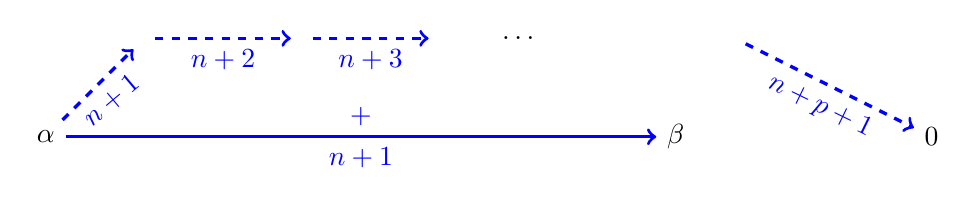
\begin{tikzpicture}[very thick, scale=0.25]
\node (alpha) at (0,0) {$\alpha$};
    \node (beta) at (32, 0){$\beta$};
  

  \draw[->, very thick,blue] (alpha)-- node [below]{$n+1$} node [above] {$+$} (beta);

  \node (alpha1) at (5,5) {};
  \node (alpha2) at (13,5) {};
    \node (alpha3) at (20,5) {};
  \node (alphalast) at (35,5) {};
  \node (zero) at (45,0) {$0$};
  \draw [->, dashed,very thick,blue] (alpha)-- node [below, rotate=40]{$n+1$}  (alpha1);
  \draw [->, dashed,very thick,blue] (alpha1)-- node [below]{$n+2$}  (alpha2);
   \draw [->, dashed,very thick,blue] (alpha2)-- node [below]{$n+3$}  (alpha3);
  
  \node (dots) at (24,5) {$\dots$};
  \draw [->, dashed, very thick,blue] (alphalast)-- node [below, rotate=-26]{$n+p+1$}  (zero);

\end{tikzpicture}
\caption{A nice proof (1)}
  \label{fig:belle-preuve-1}
\end{figure}


\paragraph*{}




Since comparison on \texttt{T1} is decidable, one can compute the last step $\gamma$ of the standard path from $(\alpha,n+1)$  such that $\beta\leq \gamma$.
Let $l$ be the length of the path from $\alpha$ to $\gamma$.  

% We use for that purpose a function that computes the first index $i$ where $n\leq i <p$ and $P(i+1)$ is
% \texttt{false}, assuming that $P(n)=\texttt{true}$ and $P(p)=\texttt{false}$.

% \begin{Coqsrc}
% first_toggle  (P : nat -> bool) (n p : nat) :
% (n < p)%nat -> P n = true -> P p = false ->
% {l : nat | (n <= l)%nat /\ (l < p)%nat /\
%      (forall i : nat, (n <= i)%nat -> (i <= l)%nat -> P i = true) /\
%       P (S l) = false}
% \end{Coqsrc}


% \begin{Coqsrc}
% Let P (i:nat) := le_b beta (standard_fun (S n) alpha i).

% Remark Rem2 : {t: nat | standard_fun (S n) alpha t < beta}.

% Let t := proj1_sig Rem2.
%  Remark Rem04 : P 0.

% Remark Rem05 : P t = false.

% Remark Rem06 : (0 <  t)%nat.

%  Let l_def :=  first_toggle P 0 t  Rem06 Rem04 Rem05.

% Let l := proj1_sig Rem07.

% Let gamma := standard_fun (S n) alpha l.
% \end{Coqsrc}



This step of the proof is illustrated in figure~\vref{fig:belle-preuve-2}.



\begin{figure}[h]
  \centering
 

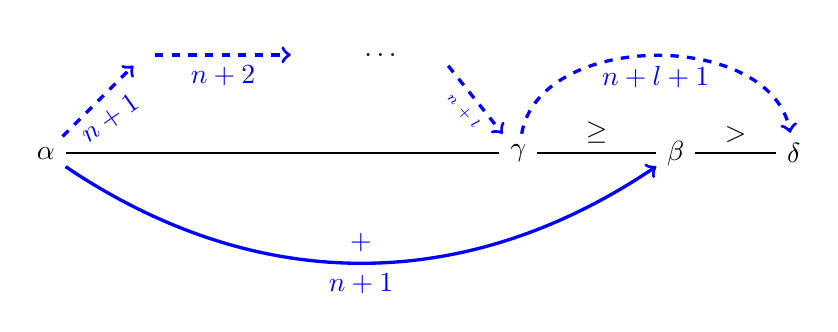
\begin{tikzpicture}[very thick, scale=0.25]
\node (alpha) at (0,0) {$\alpha$};
    \node (beta) at (32, 0){$\beta$};
  



  \node (alpha1) at (5,5) {};
  \node (alpha2) at (13,5) {};
  \node (dots) at (17,5) {$\ldots$};
    \node (alpha3) at (20,5) {};
    \node (gamma) at (24,0) {$\gamma$};
    \node (delta) at (38,0) {$\delta$};
    \draw [->, dashed,very thick,blue] (alpha)-- node [below,rotate=35]{$n+1$}  (alpha1);
  \draw [->, dashed,very thick,blue] (alpha1)-- node [below]{$n+2$}  (alpha2);
   \draw [->, dashed,very thick,blue] (alpha3)-- node [below,rotate = -48]{\tiny $n+l$}  (gamma);
   \draw  [->, dashed, blue] (gamma) to    [bend left=80] node [below]{$n+l+1$} (delta);
   \draw[->, very thick,blue] (alpha) to [bend right=34] node [below]{$n+1$} node [above] {$+$} (beta);
   \draw[thick] (alpha)--  (gamma);
   \draw[thick] (gamma)--  node [above] {$\geq$} (beta);
    \draw[thick] (beta)--  node [above] {$>$} (delta);
\end{tikzpicture}

\caption{A nice proof (2)}
  \label{fig:belle-preuve-2}
\end{figure}

\paragraph*{}

\begin{itemize}
\item If $\beta=\gamma$, its OK! We have got a standard path
from  
$\alpha$ to $\beta$ with successive indices  $n+1, n+2, \dots, n+l+1$

\item Otherwise,  $\beta < \gamma$.  Let us consider  $\delta=\canonseq{\gamma}{n+l+2}$.
By applying several times lemma \texttt{Cor12},  one converts  every path of Fig~\ref{fig:belle-preuve-2} into
 a $n+l+1$-path  (see figure~\ref{fig:belle-preuve-3}).


But $\gamma$ is on the $n+l+1$-path from $\alpha$ to $\beta$.
As shown by figure~\vref{fig:fin-belle-preuve}), the ordinal $\delta$, reachable from
$\gamma$ in one single step,  must be greater than or equal to $\beta$, which contradicts our  hypothesis $\beta < \gamma$.





\end{itemize}
 The only remaining case is  $\beta=\gamma$, thus we have got a standard path
from $\alpha$ to $\beta$.


\begin{Coqsrc}
 Lemma constant_to_standard_0 : 
    {l : nat | standard_fun (S n) alpha l = beta}.
 
End Constant_to_standard_Proof.


Lemma constant_to_standard_path 
  (alpha beta : T1) (i : nat):
  nf alpha -> const_pathS i alpha beta -> zero  < alpha ->
  {j:nat | standard_path (S i) alpha j beta}.
\end{Coqsrc}


\begin{figure}[h]
  \centering
  
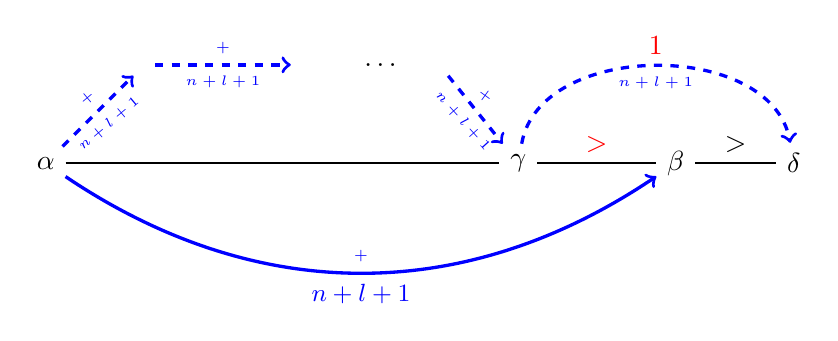
\begin{tikzpicture}[very thick, scale=0.25]
\node (alpha) at (0,0) {$\alpha$};
    \node (beta) at (32, 0){$\beta$};
    \node (alpha1) at (5,5) {};
  \node (alpha2) at (13,5) {};
  \node (dots) at (17,5) {$\ldots$};
    \node (alpha3) at (20,5) {};
    \node (gamma) at (24,0) {$\gamma$};
    \node (delta) at (38,0) {$\delta$};
     \draw [->, dashed,very thick,blue] (alpha)-- node [below, rotate = 40] {\tiny $n+l+1$}  node [above, rotate = 40]{\tiny $+$}  (alpha1);
  \draw [->, dashed,very thick,blue] (alpha1)-- node [below]{\tiny $n+l+1$} node [above]{\tiny $+$} (alpha2);
   \draw [->, dashed,very thick,blue] (alpha3)-- node [below, rotate = -48]{\tiny $n+l+1$} node [above, rotate = -36]{\tiny $+$}  (gamma);
   \draw  [->, dashed, blue] (gamma) to    [bend left=80] node [below]{\tiny $n+l+1$} node [above]{\color{red} $1$} (delta);
   \draw[->, very thick,blue] (alpha) to [bend right=34] node [below]{\small $n+l+1$} node [above] {\tiny $+$} (beta);
    \draw[thick] (gamma)--   node [above]{\color{red} $>$}(beta);
   \draw[thick] (alpha)--  (gamma);
  
    \draw[thick] (beta)--  node [above] {$>$} (delta);

  
  
\end{tikzpicture}

\caption{A nice proof (3)}
  \label{fig:belle-preuve-3}
\end{figure}


\begin{figure}[h]
  \centering
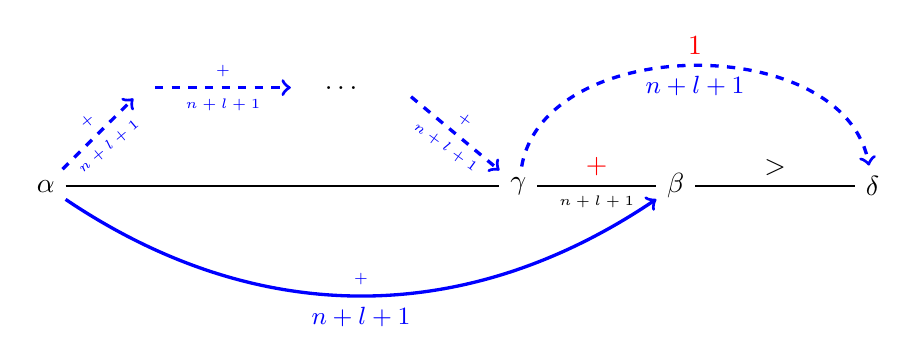
\begin{tikzpicture}[very thick, scale=0.25]
\node (alpha) at (0,0) {$\alpha$};
    \node (beta) at (32, 0){$\beta$};
  
  \node (alpha1) at (5,5) {};
  \node (alpha2) at (13,5) {};
  \node (dots) at (15,5) {$\ldots$};
    \node (alpha3) at (18,5) {};
    \node (gamma) at (24,0) {$\gamma$};
    \node (delta) at (42,0) {$\delta$};
    \draw [->, dashed,very thick,blue] (alpha)-- node [below, rotate = 40] {\tiny $n+l+1$}  node [above, rotate = 40]{\tiny $+$}  (alpha1);
  \draw [->, dashed,very thick,blue] (alpha1)-- node [below]{\tiny $n+l+1$} node [above]{\tiny $+$} (alpha2);
   \draw [->, dashed,very thick,blue] (alpha3)-- node [below, rotate = -36]{\tiny $n+l+1$} node [above, rotate = -36]{\tiny $+$}  (gamma);
   \draw  [->, dashed, blue] (gamma) to    [bend left=80] node [below]{\small $n+l+1$} node [above]{\color{red} $1$} (delta);
   \draw[->, very thick,blue] (alpha) to [bend right=34] node [below]{\small $n+l+1$} node [above] {\tiny $+$} (beta);
   \draw[thick] (alpha)--  (gamma);
  
    \draw[thick] (gamma)--  node [below]{\tiny $n+l+1$} node [above]{\color{red} $+$}(beta);
    \draw[thick] (beta)--  node [above] {$>$} (delta);

\end{tikzpicture}

\caption{A nice proof (4)}
  \label{fig:fin-belle-preuve}
\end{figure}

Applying \texttt{Lemma2\_6\_1} and \texttt{constant\_to\_standard\_path}, we get the following corollary.

\begin{Coqsrc}
Corollary  LT_to_standard_path 
      (alpha beta : T1) :
  beta   < alpha ->
  {n : nat & {j:nat | standard_path (S n) alpha j beta}}.
\end{Coqsrc}




\subsection{Back to hydras}
\label{sec:standard-battles-cases}
We are now able to complete our proof that there exists no bounded variant for proving the termination of standard hydra battles. The proof we are going to comment can
be consulted in the module 
\url{../src/html/hydras.Hydra.Epsilon0_Needed_Std.html}.
Please note that it has the same global structure as in section\ref{sec:free-battles-case} 
% ICI !
Applying the  lemmas  \texttt{Lemma2\_6\_1} of the module 
\href{../src/html/hydras.Epsilon0.Paths.html\#Lemma2_6_1}%
{\texttt{Lemma2\_6\_1}}   and 
\href{../src/html/hydras.Epsilon0.Paths.html\#constant_to_standard_path}%
{\texttt{constant\_to\_standard\_path}},
we can convert any inequality $\beta<\alpha<\epsilon_0$ into a standard path from
$\alpha$ to  $\beta$, then into a fragment of a standard battle from 
$\iota(\alpha)$ to $\iota(\beta)$.


\vspace{4pt}
\emph{From Module~\href{../src/html/hydras.Hydra.Epsilon0_Needed_Std.html\#LT_to_standard_battle}{Hydra.Epsilon0\_Needed\_Std}}

\begin{Coqsrc}
Lemma LT_to_standard_battle :
    forall alpha beta,
      beta < alpha ->
      exists n i,  fight standard  n (iota alpha) i (iota beta).
\end{Coqsrc}


Next, please consider the following context:

\begin{Coqsrc}
Section Impossibility_Proof.
 
  Context (Var : BoundedVariant standard).
 \end{Coqsrc}

In the same way as for free battles, we import a large inequality from 
the module \url{../src/html/hydras.Hydra.Epsilon0_Needed_Generic.html} .


\begin{Coqsrc}
 Lemma m_ge : m big_h <= m small_h.
\end{Coqsrc}

\paragraph*{} If remains to prove the following strict inequality, in order to have a contradiction.

\begin{Coqsrc}
Lemma m_lt : m small_h  < m big_h.
\end{Coqsrc}


\paragraph*{Proof:} Let us recall that $\texttt{big\_h} = \iota(\mu)$
 and $\texttt{small\_h} = \iota (m (\texttt{big\_h}))$.

Since $m(\texttt{big\_h })< \mu$, there exists a standard path from $\mu$ to
$m(\texttt{big\_h})$, hence a   standard battle from $\iota(\mu)$  to
$\iota(m(\texttt{big\_h}))$,  i.e. from \texttt{big\_h} to \texttt{small\_h}.

Since $m$ is assumed to be a variant for standard battles, we get the inequality  $m(\texttt{small\_h}) < m(\texttt{big\_h})$.



\subsection{Remarks}

We are grateful to 
 J. Ketonen and R. Solovay  for the high quality of their explanations and proof details.
Our proof follows tightly the sequence of lemmas in their article, with a focus on 
constructive aspects.
Roughly steaking, our implementation \emph{builds}, out of a hypothetic 
  variant $m$, bounded by some ordinal $\mu<\epsilon_0$, a hydra \texttt{big\_h} which verifies the impossible inequality  $m(\texttt{big\_h})< m(\texttt{big\_h})$.



On may ask whether the preceding results are not too restrictive, since they 
refer to a particular data type \texttt{T1}.
In fact, our representation of ordinals strictly less than 
 $\epsilon_0$ is faithful to their mathematical definition, at least 
Kurt Schütte's~\cite{schutte}, as proved in Chapter~\vref{chap:schutte}.
(please see also \href{../src/html/hydras.Schutte.Injection_E0.html}{the module \texttt{Ordinals.Schutte.Injection\_E0}}).

Thus, we can infer that our theorems can be applied to any well order.

\index{Projects}
\begin{project}
Study a possible modification of the definition of a variant  (for  standard battles).

\begin{itemize}
\item The variant is assumed to be strictly decreasing \emph{on configurations 
reachable from some initial configuration where the replication factor is equal to $0$}
\item The variant may depend on the number of the current round.
\end{itemize}

In other words, its type should be \texttt{nat -> Hydra -> T1}, and it must 
verify the inequality $m\, (S\,i)\, h' < m\,i\, h$ whenever the configuration 
$(i,h)$ is reachable from some initial configuration $(0,h_0)$
and \texttt{h} is transformed into \texttt{h'} in the considered round.
 
Can we still prove the theorems of section~\ref{std-case} with this new definition?

\end{project}


